\section{Создание приложения с использованием AngularJS}

После использования фреймворка Backbone.js было решено реализовать приложение с использование с целью выяснения практических преимуществ и недостатков.

Первым делом было решено автоматизировать развертывание приложения и воспользоваться такими средствами как npm и Bower. Npm --- это пакетный менеджер для JavaScript, который является частью проекта Node.js. Этот инструмент позволяет автоматизировать сборку приложения (с использование Bower), тестирование и развертывание. Установка не отличается ничем примечательным --- необходимо из репозиториев или же с официального сайта (http://nodejs.org) произвести установку Node.js и npm идет с ним же\cite{npm}. Все инструкции для автоматизации находятся в файле package.json. В процессе реализации данного приложения был написан следующий файл конфигурации:
\begin{lstlisting}[basicstyle=\normalsize]
{
  "name": "adhoc-project",
  "devDependencies": {
    "http-server": "^0.6.1",
    "bower": "^1.3.1"
  },
  "scripts": {
    "postinstall": "bower install",
    "prestart": "npm install",
    "start": "http-server -a 0.0.0.0 -p 8080"
  }
}
\end{lstlisting}

Такая конфигурация позволяет из командой строки выполнить:
\begin{lstlisting}
npm run
\end{lstlisting}

И произойдет следующее: установятся все необходимые зависимости для развертывания приложения, выполнится bower install и запустится веб-сервер на 8080 порту. Таким, образом, не нужно включать в проект зависимые библиотеки --- это произойдет автоматически, основываясь на конфигурации, описанной в package.json.

Для управления зависимостями JavaScript-библиотек был выбран менеджер пакетов Bower. Bower --- не стандартный менеджер пакетов, но самый популярный. Сейчас в репозитории находится более 11 тысяч пакетов\cite{bower}. Bower не навязывает пользователю свою систему сборки, а разработчику пакетов --- метод подключения библиотеки. Всё, что делает Bower --- устанавливает нужные проекту пакеты подходящих версий вместе с их зависимостями. Другими словами: просто загружает файлы нужных библиотек и всё, что нужно для их работы в специальную папку. Остальное остается на усмотрение разработчика.

После установки и настройки npm необходимо настроить конфигурацию Bower. Для этого в каталог проекта необходимо добавить файл bower.json, с содержимым которые напоминает конфигурацию npm:
\begin{lstlisting}[basicstyle=\normalsize]
{
  "name": "adhoc-project",
  "private": true,
  "dependencies": {
    "jquery": "",
    "easysoap": "",
    "bootstrap": "3.3.4",
    "angular": "~1.4.0",
    "angular-route": "~1.4.0",
    "angular-resource": "~1.4.0"
  }
}
\end{lstlisting}

% \subsection{Структура приложения}
% 
В процессе реализации данного приложения была создана следующая структура каталогов, отображенная на рисунке \ref{angular_structure}. В каталогах \textit{bower\_components} и \textit{node\_modules} хранятся библиотеки, от которых зависит данный проект. Они обновляются автоматически при помощи утилит npm и bower.
\begin{figure}[h]
\center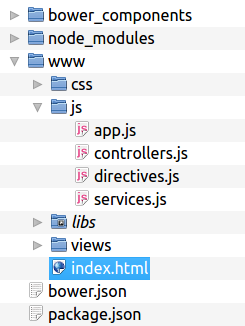
\includegraphics[width=0.4\textwidth]{angular_structure}
\caption{Структура каталогов приложения на AngularJS}\label{angular_structure}
\end{figure}

В каталоге \textit{www} хранится само приложение, где \textit{index.html} --- точка входа приложения. В каталоге \textit{css} находятся таблицы стилей, в каталоге \textit{views} шаблоны представлений. Каталог \textit{libs} представляет собой символическую ссылку на каталог bower\_components и содержит в себе необходимые проекту библиотеки.

При реализации данного проекта потребовались следующие библиотеки:
\begin{enumerate}
 \item jQuery. Библиотека JavaScript, фокусирующаяся на взаимодействии JavaScript и HTML\cite{jquery}.
 \item easySoap. WSDL SOAP клиент для JavaScript.
 \item Twitter Bootstrap. Свободный набор инструментов для создания сайтов и приложений. Включает в себя HTML и CSS шаблоны оформления\cite{bootstrap}.
 \item AngularJS. JavaScript-фреймворк предназначенный для разработки одностраничных приложений на основе MVC шаблона\cite{angular}.
\end{enumerate}

В каталоге \textit{js} находятся четыре JavaScript-скрипта, логически разделенные на различные части приложения: маршрутизация, контроллеры, директивы, сервисы:
\begin{enumerate}
 \item app.js. Описывается структура приложения: используемые модули и маршрутизация.
 \item controllers.js. Модуль, который содержит в себе все контроллеры, определенные в данном проекте.
 \item directives.js. Модуль с реализованными дополнительными директивами: для построения графика и для вывода сообщений.
 \item services.js. Модуль, в котором реализованы различные сервисы для работы с данными: получение/отправка данных на сервис по протоколу SOAP, сервис для обработки сообщений пользователю и сервис для перевода машинных идентификаторов в формат, понятный человеку.
\end{enumerate}

\subsection{Точка входа, шаблоны и представления}

Точкой входа в одностраничное приложение является файл \textit{index.html}. Это HTML страница, которая строится при помощи HTML приведенного ниже. Данный код также содержит некоторые ключевые angular директивы.
\begin{lstlisting}[basicstyle=\footnotesize]
<!doctype <!DOCTYPE html>
<html ng-app="adhocApp">
<head>
  <meta charset="utf-8">
  <title>Вероятностная система в модели AD-HOC сети</title>
  <link rel="stylesheet" href="libs/bootstrap/dist/css/bootstrap.min.css">
  <link rel="stylesheet" href="css/style.css">

  <script src="libs/jquery/dist/jquery.min.js"></script>
  <script src="libs/easysoap/easysoap.js"></script>
  <script src="libs/angular/angular.min.js"></script>
  <script src="libs/angular-route/angular-route.min.js"></script>
  <script src="libs/angular-resource/angular-resource.min.js"></script>
</head>
<body>

 <div class="container">
    <div class="row row-offcanvas row-offcanvas-right">
      <div class="col-xs-12 col-sm-9" id="content">
        <div ng-view></div>
      </div>

      <div class="col-xs-6 col-sm-3 sidebar-offcanvas" id="sidebar" role="navigation">
        <div class="list-group">
          <a href="#new" class="list-group-item">Новое исследование</a>
          <a href="#issue" class="list-group-item">Список проведенных исследований</a>
        </div>
      </div>
    </div>
</div>

<script src="js/app.js"></script>
<script src="js/controllers.js"></script>
<script src="js/services.js"></script>
<script src="js/directives.js"></script>
</body>
</html> 
\end{lstlisting}
Директива ng-app используется как флаг, который сообщает Angular-у корневой элемент нашего приложения. Это позволяет определить всю HTML-страницу как Angular-приложение. При загрузке приложения происходит автоматическая инициализация при помощи директивы ngApp.

В разделе \textit{head} определены сторонние библиотеки, без которых невозможна работа данного приложения. В разделе \textit{body} описывается основная структура приложения с использованием Twitter Bootstrap. Создается колоночный макет, состоящий из двух колонок: содержимое страницы и навигация.

Отображение содержимого страницы происходит при помощи директивы ngView. После этапа инициализации приложения, Angular создаёт инжектор, который будет использован во всем приложении, подгружаются необходимые зависимости, и происходит компиляция DOM. И директива ngView позволяет включать в себя шаблон текущего представления. Это возможно потому, что Angular поддерживает частичные представления и это позволяет отлично отделять логику от представления.

HTML отлично подходит для описания статичных документов, но теряет свою эффективность при попытке описать динамические виды в веб-приложениях. AngularJS позволяет расширить синтаксис HTML. В результате код получается выразительным, читаемым, и легко поддерживается.

Другие фреймворки обходят недостатки HTML либо абстрагируясь от HTML, CSS или JavaScript, либо навязывая обязательные инструменты для манипулирования DOM. Ни один из этих способов ни устраняет суть проблемы, а именно то, что HTML не предназначен для динамических приложений.

В Angular'е, представление (view) это проекция модели (model) через HTML-шаблон (template). Это означает, что всякий раз, когда модель изменяется, Angular обновляет соответствующие связывания (binding points), которые обновляют представление (view). Представление (view) строится Angular`ом из шаблона. Шаблоны для данного проекта помещены в каталог \textit{views} и подгружаются при необходимости. Шаблоны использовались те же, что и в приложении на Backbone.js и были адаптированы специально под AngularJS. Вместо шаблонизатора использовались определенные директивы, но сам стиль приложения остался тот же. Исходные коды шаблонов представлены в приложении А.

\subsection{Маршрутизация и контроллеры}

Все приложения в AngularJS создаются через модули. Модуль может зависеть от других, или быть одиночным. Модули служат контейнерами для разных разделов приложения, таким образом делая код пригодным для повторного использования. Для создания модуля применяется глобальный Object, пространство имен фреймворка, и метод module:
\begin{lstlisting}[basicstyle=\normalsize]
var adhocApp = angular.module('adhocApp', [
  'ngRoute',
  'adhocControllers',
  'adhocServices',
  'adhocDirectives'
]);
\end{lstlisting}

Первым параметром указывается название модуля, вторым аргументом идет список зависимостей модуля, которые также нужно подключить. Модули могут зависеть от других модулей, которые в свою очередь тоже могут иметь зависимости.
Инициализация AngularJS приложения происходит автоматически, используя директиву ngApp. Затем инициализируется Инжектор, который будет использоваться для внедрения зависимости (dependency injection) в рамках создания приложения. Инжектор будет создавать корневую область видимости (root scope), которая станет контекстом для модели нашего приложения. Angular будет"компилировать DOM, начиная с корневого элемента ngApp, подготавливая найденные директивы и связывая директивы с соответствующими элементами\cite{angular:tutorial}.

Маршруты в Angular задаются с помощью \$routeProvider'а, который предоставляет сервис \$route. Этот сервис позволяет легко связывать воедино контроллеры, шаблоны представления и текущий URL браузера:
\begin{lstlisting}[basicstyle=\normalsize]
$routeProvider.
  when('/issue', {
    templateUrl: 'views/issue-list.html',
    controller: 'IssueListController'
  }).
  when('/new', {
    templateUrl: 'views/new-issue.html',
    controller: 'AlgorithmController'
  }).
  when('/issue/:id', {
    templateUrl: 'views/result.html',
    controller: 'ResultController'
  }).
  otherwise({
    redirectTo: '/issue'
  });
\end{lstlisting}

Контроллер Angular сводит вместе бизнес-логику и логику представления. Контроллер принимает два аргумента – имя, по которому на него можно ссылаться, и функцию описывающее поведение контроллера:
\begin{lstlisting}[basicstyle=\normalsize]
angular
  .module('adhocControllers', [])
  .controller('IssueListController', ['$scope', 'Results', IssueListController]);

function IssueListController($scope, Results) {
  Results.query()
    .$promise.then(function (result) {
      angular.forEach(result, function(index) {
        var name = index.algorithm + '. ';
        name += index.area + ', ';
        name += '' + index.size + ', ' + index.step;
        index.name = name;
      });
      $scope.issues = result;
  });
}
\end{lstlisting}

Контроллер общается с Сервисом, и передает данные в том же, или измененном формате в наш Вид через объект \$scope. Когда Вид обновлён, логика Контроллера также обновляется, и её можно передавать обратно на сервер через Сервис. Благодаря двухстороннему связыванию, любые изменения, внесенные в модель отражаются в представлении, любые изменения, которые происходят в представлении отражаются в модели. Остальные контроллеры идентичны контроллерам в Backbone.js и были адаптированы под использование в AngularJS. Исходные коды отображены в приложении В.


